\documentclass[]{article}
\usepackage{lmodern}
\usepackage{amssymb,amsmath}
\usepackage{ifxetex,ifluatex}
\usepackage{fixltx2e} % provides \textsubscript
\ifnum 0\ifxetex 1\fi\ifluatex 1\fi=0 % if pdftex
  \usepackage[T1]{fontenc}
  \usepackage[utf8]{inputenc}
\else % if luatex or xelatex
  \ifxetex
    \usepackage{mathspec}
  \else
    \usepackage{fontspec}
  \fi
  \defaultfontfeatures{Ligatures=TeX,Scale=MatchLowercase}
\fi
% use upquote if available, for straight quotes in verbatim environments
\IfFileExists{upquote.sty}{\usepackage{upquote}}{}
% use microtype if available
\IfFileExists{microtype.sty}{%
\usepackage{microtype}
\UseMicrotypeSet[protrusion]{basicmath} % disable protrusion for tt fonts
}{}
\usepackage[margin=1in]{geometry}
\usepackage{hyperref}
\hypersetup{unicode=true,
            pdftitle={Yellowstone Birds},
            pdfauthor={Luna L. Sánchez-Reyes and Brian O'Meara},
            pdfborder={0 0 0},
            breaklinks=true}
\urlstyle{same}  % don't use monospace font for urls
\usepackage{color}
\usepackage{fancyvrb}
\newcommand{\VerbBar}{|}
\newcommand{\VERB}{\Verb[commandchars=\\\{\}]}
\DefineVerbatimEnvironment{Highlighting}{Verbatim}{commandchars=\\\{\}}
% Add ',fontsize=\small' for more characters per line
\usepackage{framed}
\definecolor{shadecolor}{RGB}{248,248,248}
\newenvironment{Shaded}{\begin{snugshade}}{\end{snugshade}}
\newcommand{\AlertTok}[1]{\textcolor[rgb]{0.94,0.16,0.16}{#1}}
\newcommand{\AnnotationTok}[1]{\textcolor[rgb]{0.56,0.35,0.01}{\textbf{\textit{#1}}}}
\newcommand{\AttributeTok}[1]{\textcolor[rgb]{0.77,0.63,0.00}{#1}}
\newcommand{\BaseNTok}[1]{\textcolor[rgb]{0.00,0.00,0.81}{#1}}
\newcommand{\BuiltInTok}[1]{#1}
\newcommand{\CharTok}[1]{\textcolor[rgb]{0.31,0.60,0.02}{#1}}
\newcommand{\CommentTok}[1]{\textcolor[rgb]{0.56,0.35,0.01}{\textit{#1}}}
\newcommand{\CommentVarTok}[1]{\textcolor[rgb]{0.56,0.35,0.01}{\textbf{\textit{#1}}}}
\newcommand{\ConstantTok}[1]{\textcolor[rgb]{0.00,0.00,0.00}{#1}}
\newcommand{\ControlFlowTok}[1]{\textcolor[rgb]{0.13,0.29,0.53}{\textbf{#1}}}
\newcommand{\DataTypeTok}[1]{\textcolor[rgb]{0.13,0.29,0.53}{#1}}
\newcommand{\DecValTok}[1]{\textcolor[rgb]{0.00,0.00,0.81}{#1}}
\newcommand{\DocumentationTok}[1]{\textcolor[rgb]{0.56,0.35,0.01}{\textbf{\textit{#1}}}}
\newcommand{\ErrorTok}[1]{\textcolor[rgb]{0.64,0.00,0.00}{\textbf{#1}}}
\newcommand{\ExtensionTok}[1]{#1}
\newcommand{\FloatTok}[1]{\textcolor[rgb]{0.00,0.00,0.81}{#1}}
\newcommand{\FunctionTok}[1]{\textcolor[rgb]{0.00,0.00,0.00}{#1}}
\newcommand{\ImportTok}[1]{#1}
\newcommand{\InformationTok}[1]{\textcolor[rgb]{0.56,0.35,0.01}{\textbf{\textit{#1}}}}
\newcommand{\KeywordTok}[1]{\textcolor[rgb]{0.13,0.29,0.53}{\textbf{#1}}}
\newcommand{\NormalTok}[1]{#1}
\newcommand{\OperatorTok}[1]{\textcolor[rgb]{0.81,0.36,0.00}{\textbf{#1}}}
\newcommand{\OtherTok}[1]{\textcolor[rgb]{0.56,0.35,0.01}{#1}}
\newcommand{\PreprocessorTok}[1]{\textcolor[rgb]{0.56,0.35,0.01}{\textit{#1}}}
\newcommand{\RegionMarkerTok}[1]{#1}
\newcommand{\SpecialCharTok}[1]{\textcolor[rgb]{0.00,0.00,0.00}{#1}}
\newcommand{\SpecialStringTok}[1]{\textcolor[rgb]{0.31,0.60,0.02}{#1}}
\newcommand{\StringTok}[1]{\textcolor[rgb]{0.31,0.60,0.02}{#1}}
\newcommand{\VariableTok}[1]{\textcolor[rgb]{0.00,0.00,0.00}{#1}}
\newcommand{\VerbatimStringTok}[1]{\textcolor[rgb]{0.31,0.60,0.02}{#1}}
\newcommand{\WarningTok}[1]{\textcolor[rgb]{0.56,0.35,0.01}{\textbf{\textit{#1}}}}
\usepackage{longtable,booktabs}
\usepackage{graphicx,grffile}
\makeatletter
\def\maxwidth{\ifdim\Gin@nat@width>\linewidth\linewidth\else\Gin@nat@width\fi}
\def\maxheight{\ifdim\Gin@nat@height>\textheight\textheight\else\Gin@nat@height\fi}
\makeatother
% Scale images if necessary, so that they will not overflow the page
% margins by default, and it is still possible to overwrite the defaults
% using explicit options in \includegraphics[width, height, ...]{}
\setkeys{Gin}{width=\maxwidth,height=\maxheight,keepaspectratio}
\IfFileExists{parskip.sty}{%
\usepackage{parskip}
}{% else
\setlength{\parindent}{0pt}
\setlength{\parskip}{6pt plus 2pt minus 1pt}
}
\setlength{\emergencystretch}{3em}  % prevent overfull lines
\providecommand{\tightlist}{%
  \setlength{\itemsep}{0pt}\setlength{\parskip}{0pt}}
\setcounter{secnumdepth}{5}
% Redefines (sub)paragraphs to behave more like sections
\ifx\paragraph\undefined\else
\let\oldparagraph\paragraph
\renewcommand{\paragraph}[1]{\oldparagraph{#1}\mbox{}}
\fi
\ifx\subparagraph\undefined\else
\let\oldsubparagraph\subparagraph
\renewcommand{\subparagraph}[1]{\oldsubparagraph{#1}\mbox{}}
\fi

%%% Use protect on footnotes to avoid problems with footnotes in titles
\let\rmarkdownfootnote\footnote%
\def\footnote{\protect\rmarkdownfootnote}

%%% Change title format to be more compact
\usepackage{titling}

% Create subtitle command for use in maketitle
\providecommand{\subtitle}[1]{
  \posttitle{
    \begin{center}\large#1\end{center}
    }
}

\setlength{\droptitle}{-2em}

  \title{Yellowstone Birds}
    \pretitle{\vspace{\droptitle}\centering\huge}
  \posttitle{\par}
    \author{Luna L. Sánchez-Reyes and Brian O'Meara}
    \preauthor{\centering\large\emph}
  \postauthor{\par}
      \predate{\centering\large\emph}
  \postdate{\par}
    \date{2019-09-30}


\begin{document}
\maketitle

This is an example to use rphylotastic tools to contextualize phylogenetic relationships.
The main packages are not yet installable via CRAN, so to install them you have to use the \texttt{install\_github} function from the package \texttt{devtools}:

\begin{Shaded}
\begin{Highlighting}[]
\KeywordTok{install.packages}\NormalTok{(}\StringTok{"devtools"}\NormalTok{) }\CommentTok{# this installs devtools package}
\KeywordTok{library}\NormalTok{(devtools) }\CommentTok{# this loads the package contents into the workspace}
\CommentTok{# the following two lines install datelife and rphylotastic from development repositories}
\KeywordTok{install_github}\NormalTok{(}\StringTok{"phylotastic/datelife"}\NormalTok{) }
\KeywordTok{install_github}\NormalTok{(}\StringTok{"phylotastic/rphylotastic"}\NormalTok{)}
\end{Highlighting}
\end{Shaded}

\begin{Shaded}
\begin{Highlighting}[]
\KeywordTok{library}\NormalTok{(datelife)}
\KeywordTok{library}\NormalTok{(rphylotastic)}
\end{Highlighting}
\end{Shaded}

Now, say you are hiking in Yellowstone with ypur students, and yu want them to get the phylogenetic relationships of the organisms they spotted during the hike.
The function \texttt{taxa\_common\_to\_sicentific} will get the scientific names from common names you provide. In this example, the student is interested in birds:

\begin{Shaded}
\begin{Highlighting}[]
\NormalTok{birds_I_saw =}\StringTok{ }\KeywordTok{taxa_common_to_scientific}\NormalTok{(}\KeywordTok{c}\NormalTok{(}\StringTok{"Osprey"}\NormalTok{, }\StringTok{"House sparrow"}\NormalTok{, }
    \StringTok{"Mallard duck"}\NormalTok{, }\StringTok{"American Robin"}\NormalTok{, }\StringTok{"song sparrow"}\NormalTok{, }\StringTok{"mourning dove"}\NormalTok{, }
    \StringTok{"house wren"}\NormalTok{))}
\end{Highlighting}
\end{Shaded}

This gets the species that will provide phylogenetic context to the focal species:

\begin{Shaded}
\begin{Highlighting}[]
\NormalTok{yellowstone_birds <-}\StringTok{ }\KeywordTok{url_get_scientific_names}\NormalTok{(}\DataTypeTok{URL=}
    \StringTok{"https://www.nps.gov/yell/learn/nature/upload/BirdChecklist2014.pdf"}\NormalTok{)}
\end{Highlighting}
\end{Shaded}

Then, we will get the tree with dates containing both the focal species and their phylogenetic context

\begin{Shaded}
\begin{Highlighting}[]
\NormalTok{yellowstone_bird_tree <-}\StringTok{ }\NormalTok{datelife}\OperatorTok{::}\KeywordTok{datelife_search}\NormalTok{(}
    \KeywordTok{taxa_get_otol_tree}\NormalTok{(yellowstone_birds), summary_format }
\NormalTok{    =}\StringTok{ "phylo_median"}\NormalTok{)}
\end{Highlighting}
\end{Shaded}

To plot the tree you will need some \texttt{ape} package functions:

\begin{Shaded}
\begin{Highlighting}[]
\KeywordTok{library}\NormalTok{(ape)}
\end{Highlighting}
\end{Shaded}

\begin{Shaded}
\begin{Highlighting}[]
\KeywordTok{par}\NormalTok{(}\DataTypeTok{xpd =} \OtherTok{NA}\NormalTok{)}
\NormalTok{ape}\OperatorTok{::}\KeywordTok{plot.phylo}\NormalTok{(yellowstone_bird_tree,}
      \DataTypeTok{tip.color =} \KeywordTok{ifelse}\NormalTok{(yellowstone_bird_tree}\OperatorTok{$}\NormalTok{tip.label}\OperatorTok\NormalTok{birds_I_saw, }\StringTok{"red"}\NormalTok{, }\StringTok{"black"}\NormalTok{),}
      \DataTypeTok{cex=}\FloatTok{0.3}\NormalTok{, }\DataTypeTok{type =} \StringTok{"fan"}\NormalTok{, }\DataTypeTok{edge.width =} \FloatTok{0.45}\NormalTok{, }\DataTypeTok{label.offset =} \FloatTok{1.5}\NormalTok{)}
\end{Highlighting}
\end{Shaded}

\begin{center}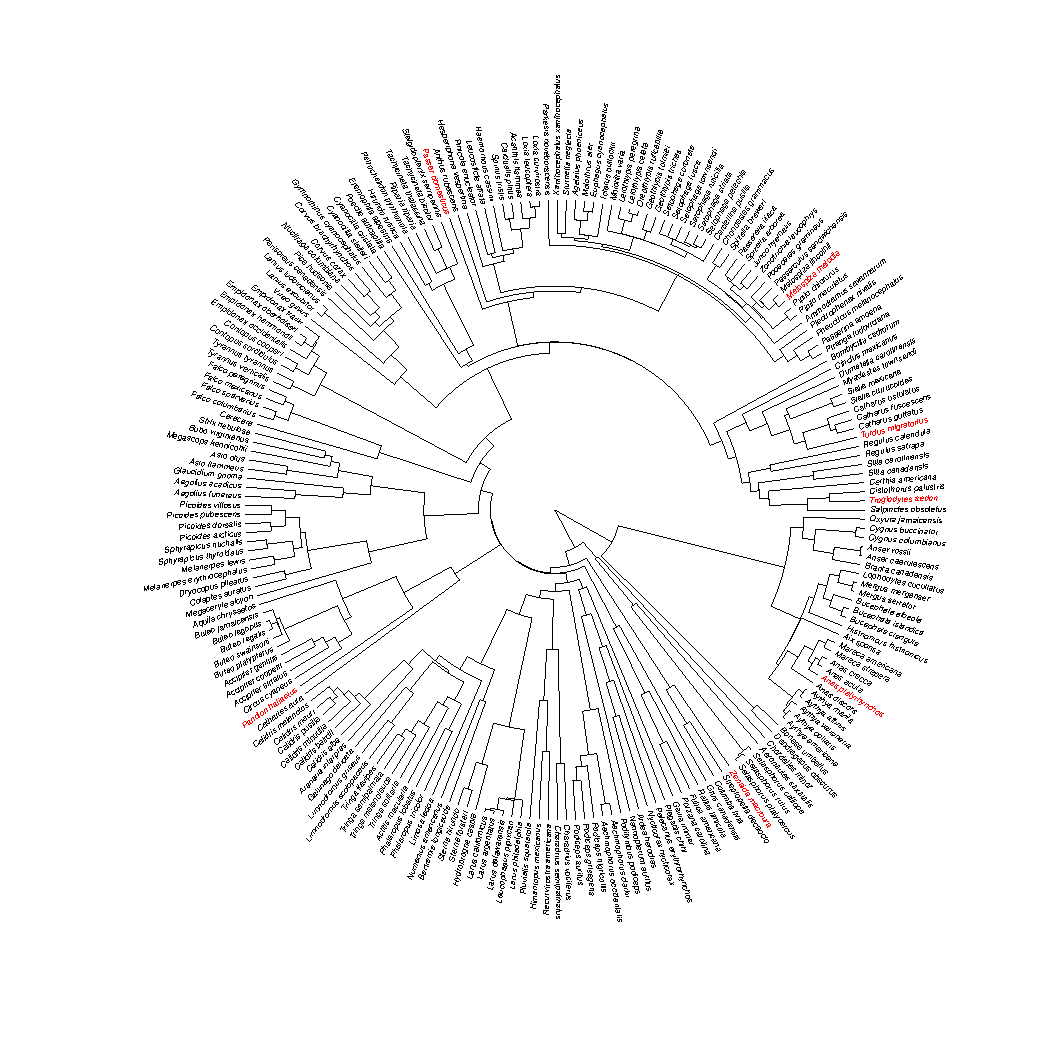
\includegraphics[width=\textwidth]{yellowstone_birds_files/figure-latex/unnamed-chunk-6-1} \end{center}

We can add taxonomic labels such as family names. If you have a table with the corresponding families to each species on the tip of the tree, you can type it in as a vector, or read it with \texttt{read.table} function.
If you do not have that info, you can pull it using a \texttt{datelife} function called \texttt{get\_ott\_clade}.

\begin{Shaded}
\begin{Highlighting}[]
\NormalTok{yellowstone_bird_fams =}\StringTok{ }\KeywordTok{get_ott_clade}\NormalTok{(}\DataTypeTok{ott_ids =}\NormalTok{ yellowstone_bird_tree}\OperatorTok{$}\NormalTok{ott_ids,}
        \DataTypeTok{ott_rank =} \StringTok{"family"}\NormalTok{)}
\end{Highlighting}
\end{Shaded}

Then, we will make a list of species within families, to feed to the function that will plot the arcs:
We will call this list \texttt{tipsies}

\begin{Shaded}
\begin{Highlighting}[]
\NormalTok{families =}\StringTok{ }\KeywordTok{unique}\NormalTok{(}\KeywordTok{names}\NormalTok{(yellowstone_bird_fams}\OperatorTok{$}\NormalTok{family))}
\NormalTok{tipsies =}\StringTok{ }\KeywordTok{sapply}\NormalTok{(families, }\ControlFlowTok{function}\NormalTok{(x) }
\NormalTok{    yellowstone_bird_tree}\OperatorTok{$}\NormalTok{tip.label[}\KeywordTok{names}\NormalTok{(yellowstone_bird_fams}\OperatorTok{$}\NormalTok{family)}\OperatorTok\NormalTok{x])}
\end{Highlighting}
\end{Shaded}

Now we are gonna set the colors of the arc lines in the variable \texttt{arc\_grays} and their position in \texttt{arc\_line\_offset}:

\begin{Shaded}
\begin{Highlighting}[]
\NormalTok{seede =}\StringTok{ }\KeywordTok{set.seed}\NormalTok{(}\DecValTok{100}\NormalTok{)}
\NormalTok{arc_grays =}\StringTok{ }\KeywordTok{sample}\NormalTok{(}\KeywordTok{gray.colors}\NormalTok{(}\DataTypeTok{n =} \KeywordTok{length}\NormalTok{(tipsies)), }\KeywordTok{length}\NormalTok{(tipsies))}
\NormalTok{arc_line_offset =}\StringTok{ }\KeywordTok{rep}\NormalTok{(}\FloatTok{1.63}\NormalTok{, }\KeywordTok{length}\NormalTok{(tipsies))}
\end{Highlighting}
\end{Shaded}

Finally, we need to costumize the position of family name labels so they do not overlap.
For that we made a function that simply adds to the already known position of the arc lines in \texttt{arc\_line\_offset}.
And then we ended up tweaking the position for certain families that were overlapping too much

\begin{Shaded}
\begin{Highlighting}[]
\NormalTok{get_arc_label_offset <-}\StringTok{ }\ControlFlowTok{function}\NormalTok{(alineo)\{}
\NormalTok{    res <-}\StringTok{ }\NormalTok{alineo }\OperatorTok{+}\StringTok{ }\FloatTok{0.05}
\NormalTok{    res[}\DecValTok{29}\NormalTok{] <-}\StringTok{ }\NormalTok{res[}\DecValTok{29}\NormalTok{]}\OperatorTok{-}\FloatTok{0.0} \CommentTok{#laridae}
\NormalTok{    res[}\DecValTok{30}\NormalTok{] <-}\StringTok{ }\NormalTok{res[}\DecValTok{30}\NormalTok{]}\OperatorTok{+}\FloatTok{0.05}
\NormalTok{    res[}\DecValTok{31}\NormalTok{] <-}\StringTok{ }\NormalTok{res[}\DecValTok{31}\NormalTok{]}\OperatorTok{-}\FloatTok{0.18} \CommentTok{#recurvirostridae}
\NormalTok{    res[}\DecValTok{34}\NormalTok{] <-}\StringTok{ }\NormalTok{res[}\DecValTok{34}\NormalTok{]}\OperatorTok{-}\FloatTok{0.16} \CommentTok{#ardeidae}
\NormalTok{    res[}\DecValTok{37}\NormalTok{] <-}\StringTok{ }\NormalTok{res[}\DecValTok{37}\NormalTok{]}\OperatorTok{-}\FloatTok{0.19} \CommentTok{#gaviidae}
    \KeywordTok{return}\NormalTok{(res)}
\NormalTok{\}}
\NormalTok{arc_label_offset =}\StringTok{ }\KeywordTok{get_arc_label_offset}\NormalTok{(arc_line_offset)}
\end{Highlighting}
\end{Shaded}

We also made a function to customize the degrees for the labels so they do not overlap. Index gives the position of he family that we want to set, and degree gives the degree that we want to set:

\begin{Shaded}
\begin{Highlighting}[]
\NormalTok{make_label_degree <-}\StringTok{ }\ControlFlowTok{function}\NormalTok{(length, index, degree)\{}
\NormalTok{  deg <-}\StringTok{ }\KeywordTok{rep}\NormalTok{(}\OtherTok{NA}\NormalTok{, length)}
  \ControlFlowTok{for}\NormalTok{(i }\ControlFlowTok{in} \KeywordTok{seq}\NormalTok{(}\KeywordTok{length}\NormalTok{(index)))\{}
\NormalTok{    deg[index[i]] <-}\StringTok{ }\NormalTok{degree[i]}
\NormalTok{  \}}
  \KeywordTok{return}\NormalTok{(deg)}
\NormalTok{\}}
\NormalTok{our_label_degree =}\StringTok{ }\KeywordTok{make_label_degree}\NormalTok{(}\KeywordTok{length}\NormalTok{(families),}
  \DataTypeTok{index =} \KeywordTok{c}\NormalTok{(}\DecValTok{5}\NormalTok{,}\DecValTok{6}\NormalTok{,}\DecValTok{7}\NormalTok{,}\DecValTok{14}\NormalTok{,}\DecValTok{15}\NormalTok{, }\DecValTok{17}\NormalTok{, }\DecValTok{31}\NormalTok{, }\DecValTok{32}\NormalTok{, }\DecValTok{34}\NormalTok{, }\DecValTok{36}\NormalTok{, }\DecValTok{37}\NormalTok{, }\DecValTok{38}\NormalTok{, }\DecValTok{39}\NormalTok{, }\DecValTok{40}\NormalTok{, }\DecValTok{43}\NormalTok{, }\DecValTok{44}\NormalTok{),}
  \DataTypeTok{degree =} \KeywordTok{c}\NormalTok{(}\DecValTok{24}\NormalTok{, }\DecValTok{26}\NormalTok{, }\DecValTok{28}\NormalTok{, }\FloatTok{112.5}\NormalTok{, }\FloatTok{116.5}\NormalTok{, }\DecValTok{125}\NormalTok{, }\DecValTok{270}\NormalTok{, }\DecValTok{275}\NormalTok{, }\DecValTok{278}\NormalTok{, }\DecValTok{293}\NormalTok{, }\DecValTok{285}\NormalTok{, }\DecValTok{297}\NormalTok{, }\DecValTok{301}\NormalTok{, }\DecValTok{304}\NormalTok{, }\DecValTok{314}\NormalTok{, }\DecValTok{316}\NormalTok{))}
\end{Highlighting}
\end{Shaded}

Finally we plot the tree again and add the labels with the rphylotasic function \texttt{arclabels}:

\begin{Shaded}
\begin{Highlighting}[]
\KeywordTok{par}\NormalTok{(}\DataTypeTok{xpd =} \OtherTok{TRUE}\NormalTok{, }\DataTypeTok{mai =} \KeywordTok{rep}\NormalTok{(}\DecValTok{1}\NormalTok{,}\DecValTok{4}\NormalTok{))}
\NormalTok{ape}\OperatorTok{::}\KeywordTok{plot.phylo}\NormalTok{(yellowstone_bird_tree,}
      \DataTypeTok{tip.color =} \KeywordTok{ifelse}\NormalTok{(yellowstone_bird_tree}\OperatorTok{$}\NormalTok{tip.label}\OperatorTok\NormalTok{birds_I_saw, }\StringTok{"red"}\NormalTok{, }\StringTok{"black"}\NormalTok{),}
      \DataTypeTok{cex=}\FloatTok{0.3}\NormalTok{, }\DataTypeTok{type =} \StringTok{"fan"}\NormalTok{, }\DataTypeTok{edge.width =} \FloatTok{0.45}\NormalTok{, }\DataTypeTok{label.offset =} \FloatTok{1.5}\NormalTok{)}
      \ControlFlowTok{for}\NormalTok{(i }\ControlFlowTok{in} \KeywordTok{seq}\NormalTok{(}\KeywordTok{length}\NormalTok{(tipsies)))\{}
        \CommentTok{# cat(i, families[i], "\textbackslash{}n")}
        \KeywordTok{arclabels}\NormalTok{(}\DataTypeTok{phy =}\NormalTok{ yellowstone_bird_tree, }\DataTypeTok{text =}\NormalTok{ families[i], }\DataTypeTok{tips =}\NormalTok{ tipsies[[i]],}
            \DataTypeTok{orientation =} \StringTok{"horizontal"}\NormalTok{, }\DataTypeTok{col =}\NormalTok{ arc_grays[i], }\DataTypeTok{lwd =} \DecValTok{4}\NormalTok{,}
            \DataTypeTok{lab.offset =}\NormalTok{ arc_label_offset[i], }\DataTypeTok{ln.offset =}\NormalTok{ arc_line_offset[i],}
            \DataTypeTok{cex =} \FloatTok{0.5}\NormalTok{, }\DataTypeTok{label_degree =}\NormalTok{ our_label_degree[i])}
\NormalTok{      \}}
\end{Highlighting}
\end{Shaded}

\begin{flushleft}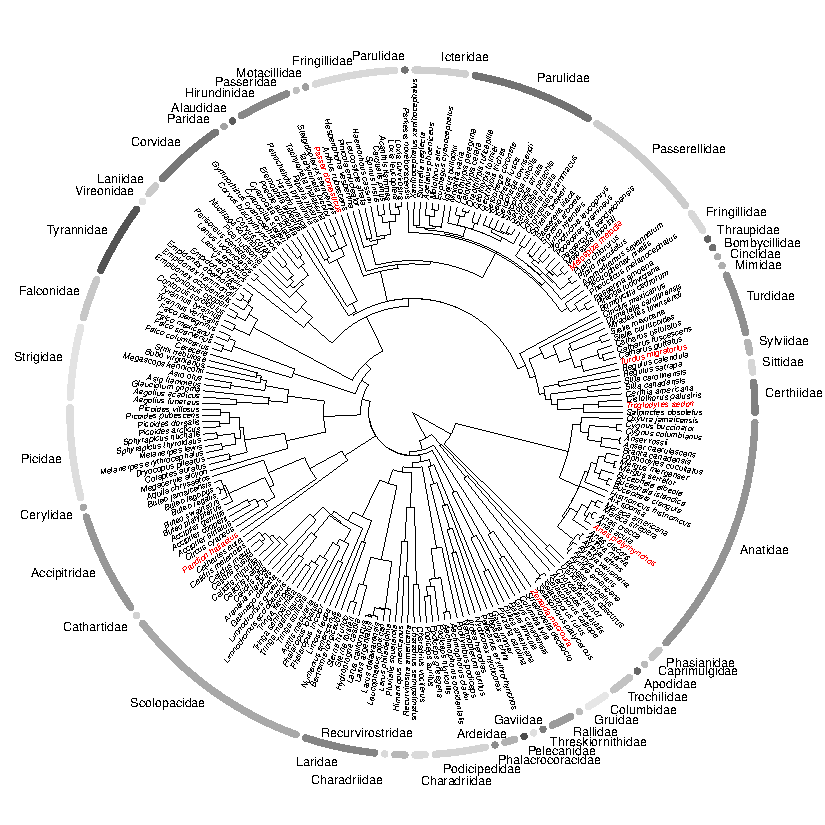
\includegraphics[width=\textwidth]{yellowstone_birds_files/figure-latex/unnamed-chunk-12-1} \end{flushleft}


\end{document}
